\chapter{Formal Analysis Using Alloy}

In this chapter is shown the use of Alloy to analyze the critical parts of the system. In particular the most crucial points to analyze are:
\begin{itemize}
	\item Only No-Tech Customer can enter with the Ticket.
	\item Customer can enter with a Line-Up or Booking Request.
	\item Customer can be involved in one started Request per time. \\
\end{itemize}
All the others Signatures and Facts are used to simplify the model in some cases or to help the building of the model in others.
In particular section 4.1 lists and explains all the Signatures used , section 4.2 all the Facts of the model and the last section 4.4 shows an example of world with Alloy's Predicates.

\section{Signatures}
This section shows the piece of code in Alloy with all the signatures used for this model.
%QUA BISOGNA DECIDERE SE FARE:

% 1 modo: SCREEN 
%\begin{figure}[H] 
%    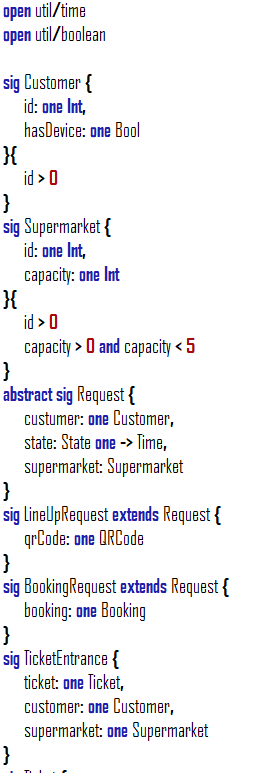
\includegraphics[scale=0.8]{./Images/ScreenAlloy/alloySig1} 
%\end{figure}

%2 modo
\begin{lstlisting} %[language=alloy, basicstyle=\small] 
//............
open util/time
open util/boolean

sig Customer {
   id: one Int,
   hasDevice: one Bool
}{
   id > 0
}
sig Supermarket {
   id: one Int,
   capacity: one Int
}{
   id > 0
}
abstract sig Request {
   custumer: one Customer,
   state: State one -> Time,
   supermarket: Supermarket
}
sig LineUpRequest extends Request {
   qrCode: one QRCode
}
sig BookingRequest extends Request {
   booking: one Booking
}
sig TicketEntrance {
   ticket: one Ticket,
   customer: one Customer,
   supermarket: one Supermarket
}
sig Ticket {
   number: one Int
}{
   number > 0
}
sig QRCode {
   id: one Int
}{
   id > 0
}
sig Booking {
   id: one Int
}{
   id > 0
}

abstract sig State {}
one sig Reserved extends State{}
one sig Started extends State{}
one sig Finished extends State{}


\end{lstlisting} 




\section{Facts}
This section shows the piece of code in Alloy that contains facts.
Some of the facts model the domain assumptions, others are needed to build a consistent model.
\begin{lstlisting} %[language=alloy, basicstyle=\small]
//............
//Unique Istances
fact uniqueQRCode {
   all disj c, c': QRCode | c.id != c'.id
}
fact uniqueBooking {
   all disj b, b': Booking | b.id != b'.id
}
fact uniqueTicket {
   all disj t, t': Ticket | t.number != t'.number
}
fact uniqueCustomer {
   all disj a, a': Customer | a.id != a'.id
}

//Only not-Tech User can have a ticket
fact ticketForNoTech {
   all t: TicketEntrance | t.customer.hasDevice = False
}
fact RequestForTechCustomer {
   all q: Request | q.custumer.hasDevice = True
}

//A QRCode, Booking, Ticket has to be associated to its Request
fact allQRCodeInLineUPRequest  {
   all q: QRCode | one l: LineUpRequest | q.id = l.qrCode.id
}
fact allBookingInBookingRequest {
   all b: Booking | one r: BookingRequest | b.id = r.booking.id
}
fact allTicketInEntrance {
   all t: Ticket | one e: TicketEntrance | t.number = e.ticket.number
}
fact requestCreationStateChart {
   //A request is always created as "Reserved"
   all r: Request | one t': Time | r.state.t' = Reserved	
}
fact requestFinishedStateChart {
   //Once a Request is finished it cannot change status again
   all r: Request, t: Time |
     (r.state.t = Finished => all t': Time | gte[t',t] => r.state.t' = Finished)	
}
fact requestStartedStateChart {
   //Once a Request is started it cannot get back to Reserved
   all r: Request, t: Time |
      (r.state.t = Started => all t': Time | gte[t',t] => r.state.t' != Reserved)	
}
//A user can be envolved in one "Started" request per time
fact oneStartedPerUser {
   no disj r,r': Request |
      r.custumer = r'.custumer and
         some t: Time |
	      r.state.t = Started and r'.state.t = Started
}
\end{lstlisting}








 
 
%\section{Assertions}
This section shows the piece of code in Alloy that contains the Assertions.  \\
\begin{lstlisting} %[language=alloy, basicstyle=\small] 
//............
assert esempioAssert{
   all ... : ...
}
\end{lstlisting}








 
 



 
 
\section{Predicates}
This section shows the piece of code in Alloy that contains the Predicates. \\

\begin{lstlisting} %[language=alloy, basicstyle=\small] 
//............
pred isCustomerInARequest[c: Customer, t: Time] {
   one r: Request | r.state.t = Started and r.custumer = c
}

pred makeALineUpRequest[c: Customer, q: QRCode, t: Time, r': LineUpRequest]{
   //precondition
   not isCustomerInARequest[c,t]
   //postcondition
   r'.custumer = c
   r'.qrCode = q
   r'.state.t = Reserved
}
run makeALineUpRequest

pred makeABookingRequest[c: Customer, b: Booking, t: Time, r': Request]{
   //precondition
   not isCustomerInARequest[c,t]
   //postcondition
   r'.custumer = c
   r'.booking = b
   r'.state.t = Reserved
}
run makeABookingRequest

pred startARequest[r: Request, t: Time]{
   //precondition
   not isCustomerInARequest[r.custumer,t]
   r.state.t = Reserved
   //postcondition
   r.state.(t.next) = Started
   isCustomerInARequest[r.custumer,t.next]
}
run startARequest

pred endARequest[r: Request, t: Time] {
   //precondition
   isCustomerInARequest[r.custumer,t]
   r.state.t = Reserved or r.state.t = Started
   //postcondition
   r.state.(t.next) = Finished
   not isCustomerInARequest[r.custumer,t.next]
}
run endARequest


//Pred Show
pred show {
   #Customer = 3
   #TicketEntrance = 1
   #BookingRequest = 1
   #LineUpRequest = 1
   #Supermarket = 1
}
run show for 3
\end{lstlisting}





 
 
\section{Generated World}
In this section it is shown the model generated by executing the Alloy code: in particular, three different Worlds are provided in order to underline the different states in which the Requests can be.
\begin{figure}[H] 
\centerline{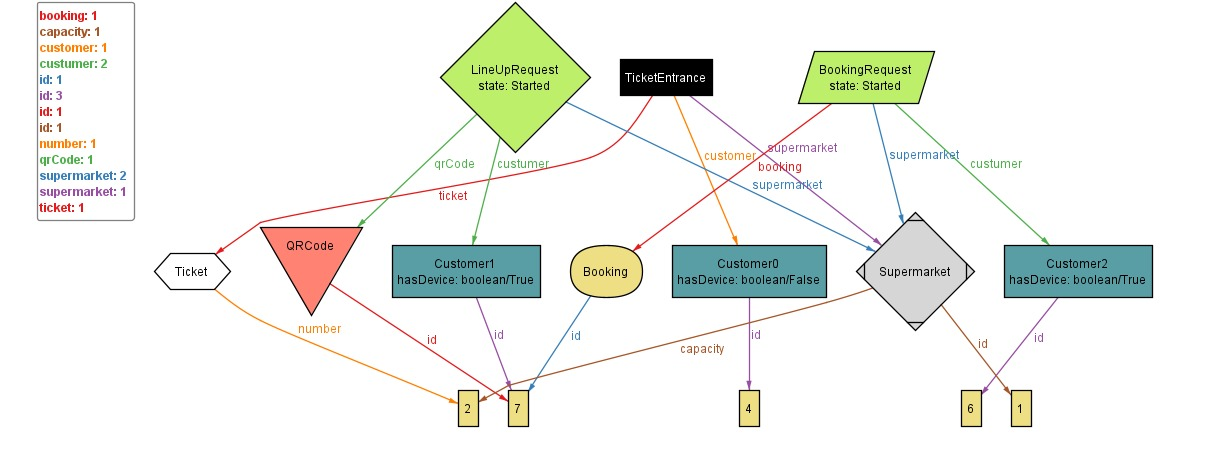
\includegraphics[scale=0.48]{world1Alloy}}
\caption{Alloy Model}
\end{figure}
\begin{figure}[H] 
\centerline{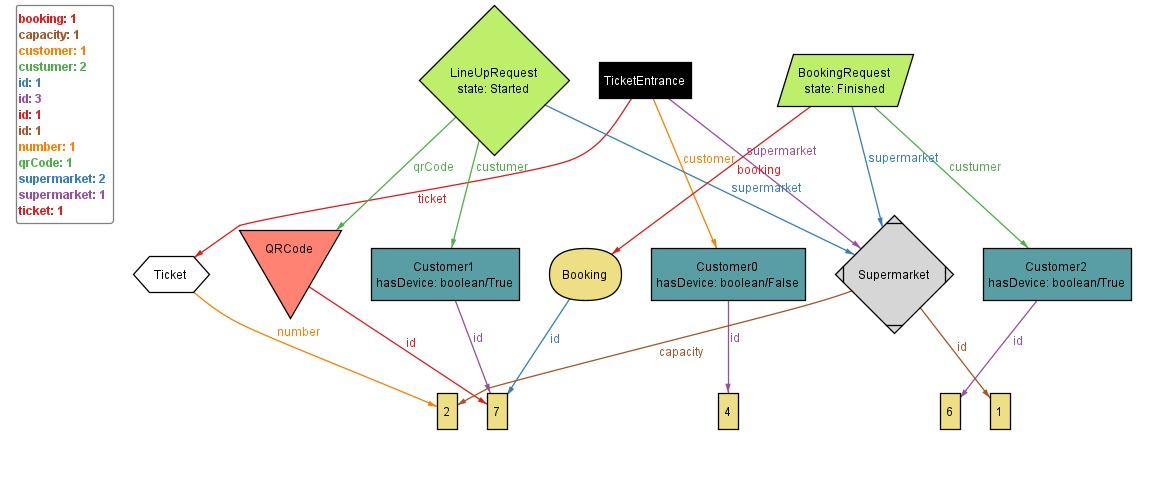
\includegraphics[scale=0.48]{world2Alloy}}
\caption{Alloy Model}
\end{figure}
\begin{figure}[H] 
\centerline{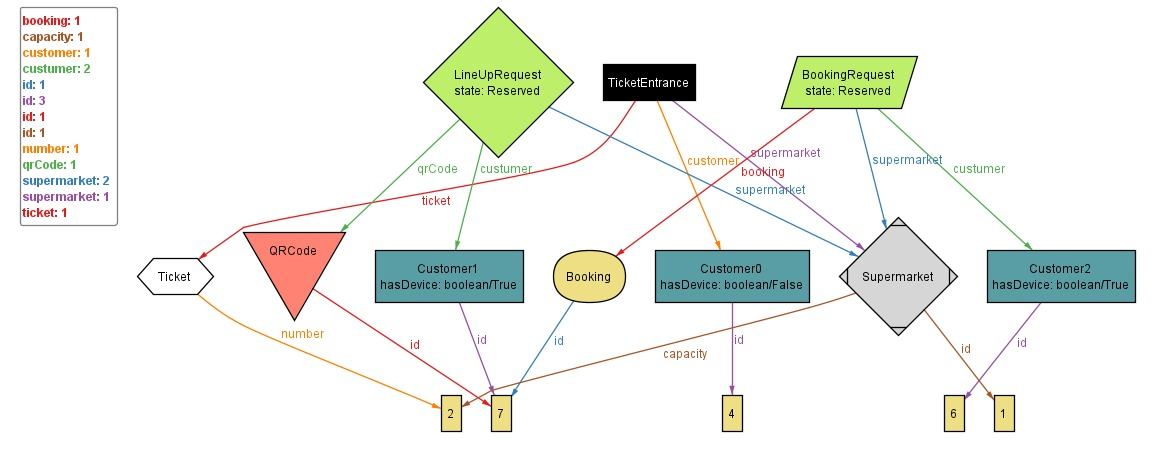
\includegraphics[scale=0.48]{world3Alloy}}
\caption{Alloy Model}
\end{figure}
\section{Proof Of Consistency}

 \begin{figure}[H]
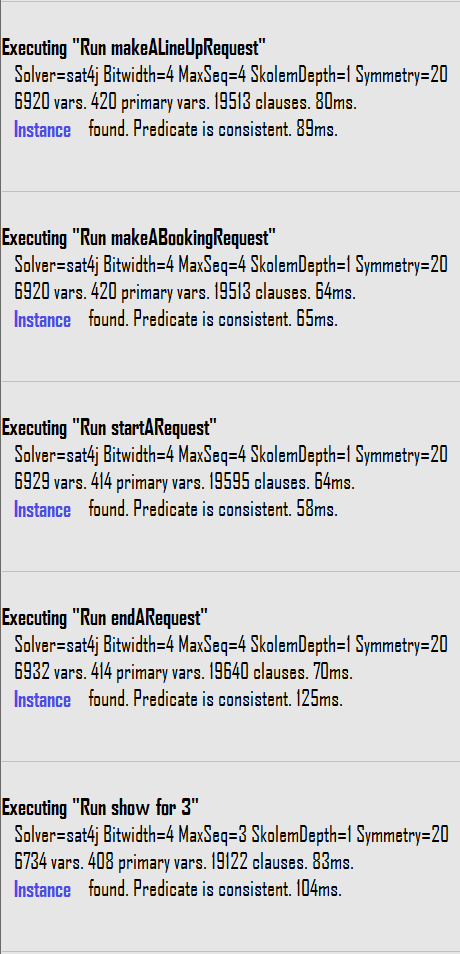
\includegraphics[scale=0.8]{./Images/ScreenAlloy/ProofOfConsistency}
\end{figure}
